\begin{section}{Resultados}

	Para analizar las diferencias y/o similitudes en la aplicación práctica de los tres algoritmos implementados se generaron gráficos que pasan a detallarse a continuación. 
		
	El primero de ellos consiste en gráficar el error relativo en función de la cantidad de iteraciones para cada uno de los algoritmos. Se utilizó precisión fija de 51 bits ya que por precondición la cantidad de dígitos de la mantisa debe ser menor a 52, es decir, con 51 dígitos minimizamos el error. Conseguimos la precisión deseada mediante truncamiento.
	El eje del gráfico que corresponde al $error\;relativo$ está en escala logarítmica para poder apreciar mejor los valores correspondientes dado que estos decrecen exponencialmente.

	\begin{figure}[H]
	  \centering
		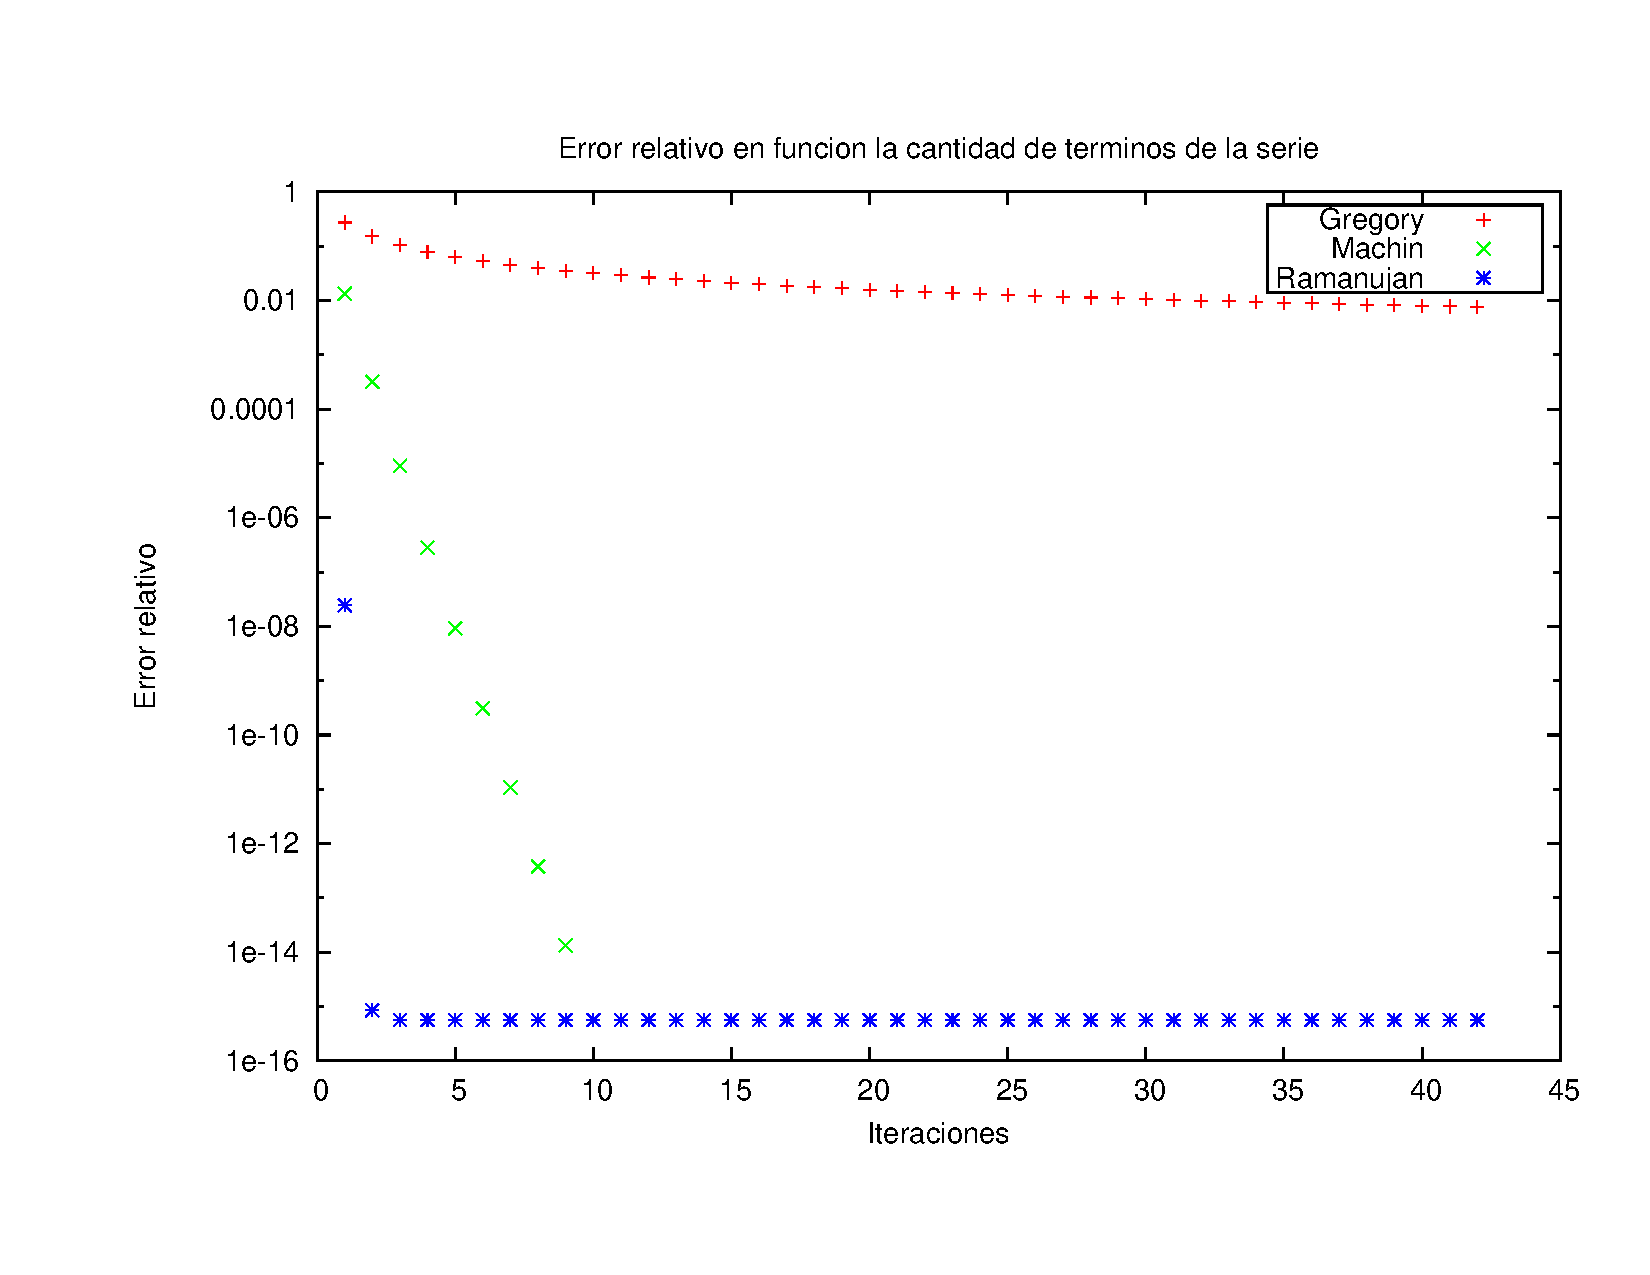
\includegraphics[width=14cm]{graficos/comparacion_1a42it_51p.pdf}
	  \caption{Comparación del error relativo de las tres series variando de 1 a 42 la cantidad de términos calculados con presición de 51 bits en la mantisa.}
	  \label{fig:51p}
	\end{figure}
	
	\VSP

	Como esperabamos observarmos en el gráfico que a medida que la cantidad de términos de la serie (cualquiera de ellas) aumenta el error cometido en el cálculo de $\pi$ disminuye.\\
	
	Observamos que el error introducido al aproximar $\pi$ con la serie de $Gregory$ es logaritmico (en escala logarítmica) en función de la cantidad de términos de la serie calculados. Lo que significa que el error de la serie de $Greory$ decrece linealmente conforme aumenta la cantidad de iteraciones.
	
	Creemos a partir del gráfico que el error relativo cometido al aproximar $\pi$ con la fórmula de $Machin$ en función de la cantidad de iteraciones es una recta con pendiente negativa. Como la escala utilizada para representar dicho error es la logarítmica, podemos decir que el error decrece exponencialmente.
	
	Además observamos que a partir de la décima iteración el gráfico no muestra de forma clara lo que ocurre con el error en la fórmula de $Machin$. Suponemos que se debe al hecho de que los valores que representan a $Machin$ se superponen con los valores correspondientes a $Ramanujan$ para esa cantidad de iteraciones.
	
	Por otro lado, podemos apreciar que con pocas iteraciones la serie de $Ramanujan$ obtiene un error constante, lo que creemos que ocurre con $Machin$ recien en la iteración diez.\\
	
	Para poder observar el comportamiento del algoritmo de $Machin$ vs. el de $Ramanujan$ a continuación se adjunta el gráfico con los mismos parámetros (51 digitos de presición), el cual muestra el error relativo entre la iteración 3 y 12.
	
	\begin{figure}[H]
	  \centering
		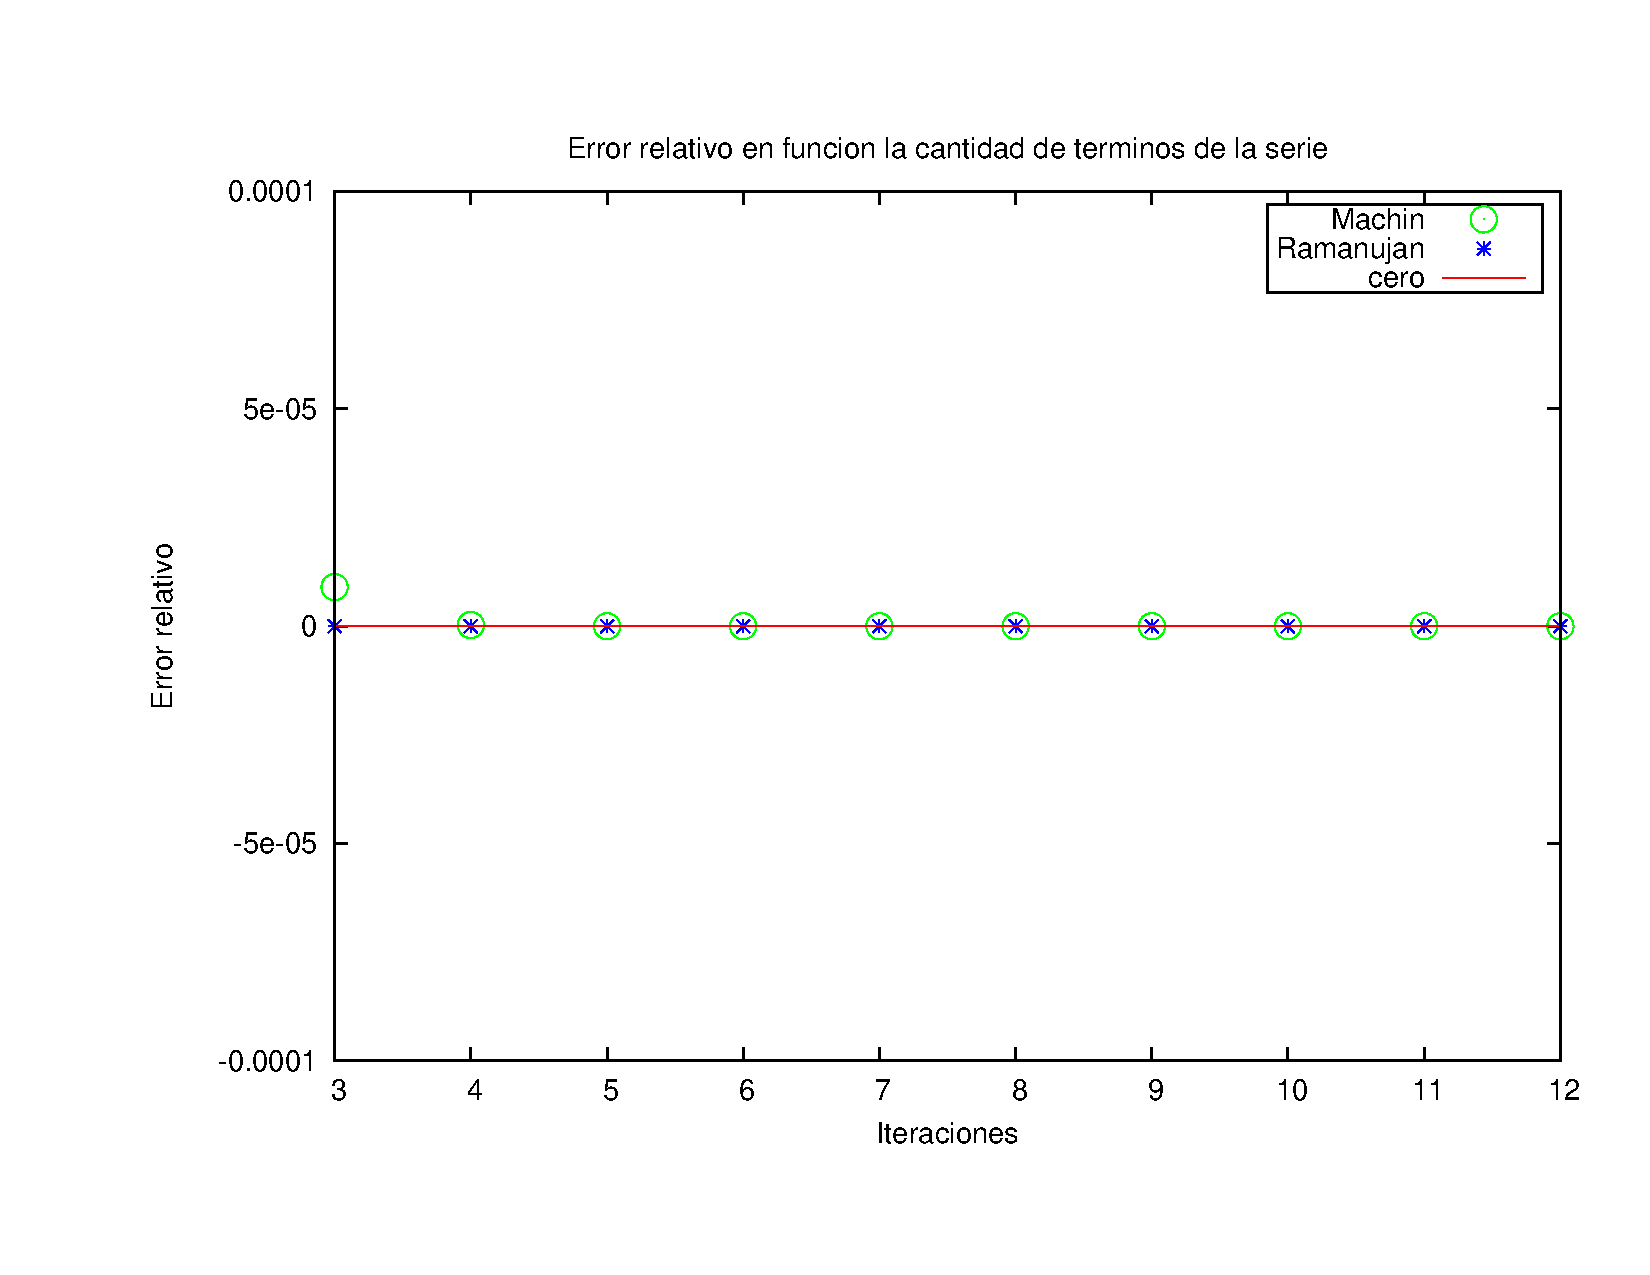
\includegraphics[width=14cm]{graficos/comparacion_machin-ram.pdf}
	  \caption{Comparación del error relativo la serie de Machin y de Ramanujan variando de 3 y 12 la cantidad de términos calculados con presición de 51 bits en la mantisa.}
	  \label{fig:greg-ram}
	\end{figure}
	
	\VSP
	
	Con este gráfico nos vemos tentados a validar lo supuesto en un principio, ya que se puede apreciar que entre estas iteraciones el error cometido por ambos métodos es el mismo. Más aun se podria concluir a partir del gráfico que el error es cero lo cual no es cierto, pero al ser un error tan chico el gráfico ayuda a la malinterpretación de los datos. Igualmente a pesar de seguir iterando no se podria obtener una mejor aproximación a $\pi$. El impedimento viene dado por la cantidad de digitos de presición utilizada.
	A partir de esto, podemos concluir que al tratarse de magnitudes tan pequeñas los gráficos son informativos en rasgos generales y no en detalles.\\	
	
	\VSP
	
	El siguiente gráfico detalla el error relativo en función de la cantidad de bits de precisión (variando este parámetro de 1 a 51).
	
	Se corrieron las pruebas hasta 42 iteraciones debido a que la serie de $Ramanujan$ es informativa hasta esa iteración (a partir de 43 iteraciones devuelve $nan$), es decir, el error relativo presentado corresponde al error cometido al calcular 42 términos de la serie.
	
	El gráfico se presenta bajo una escala logarítmica en $y$.
	
	\begin{figure}[H]
	  \centering
		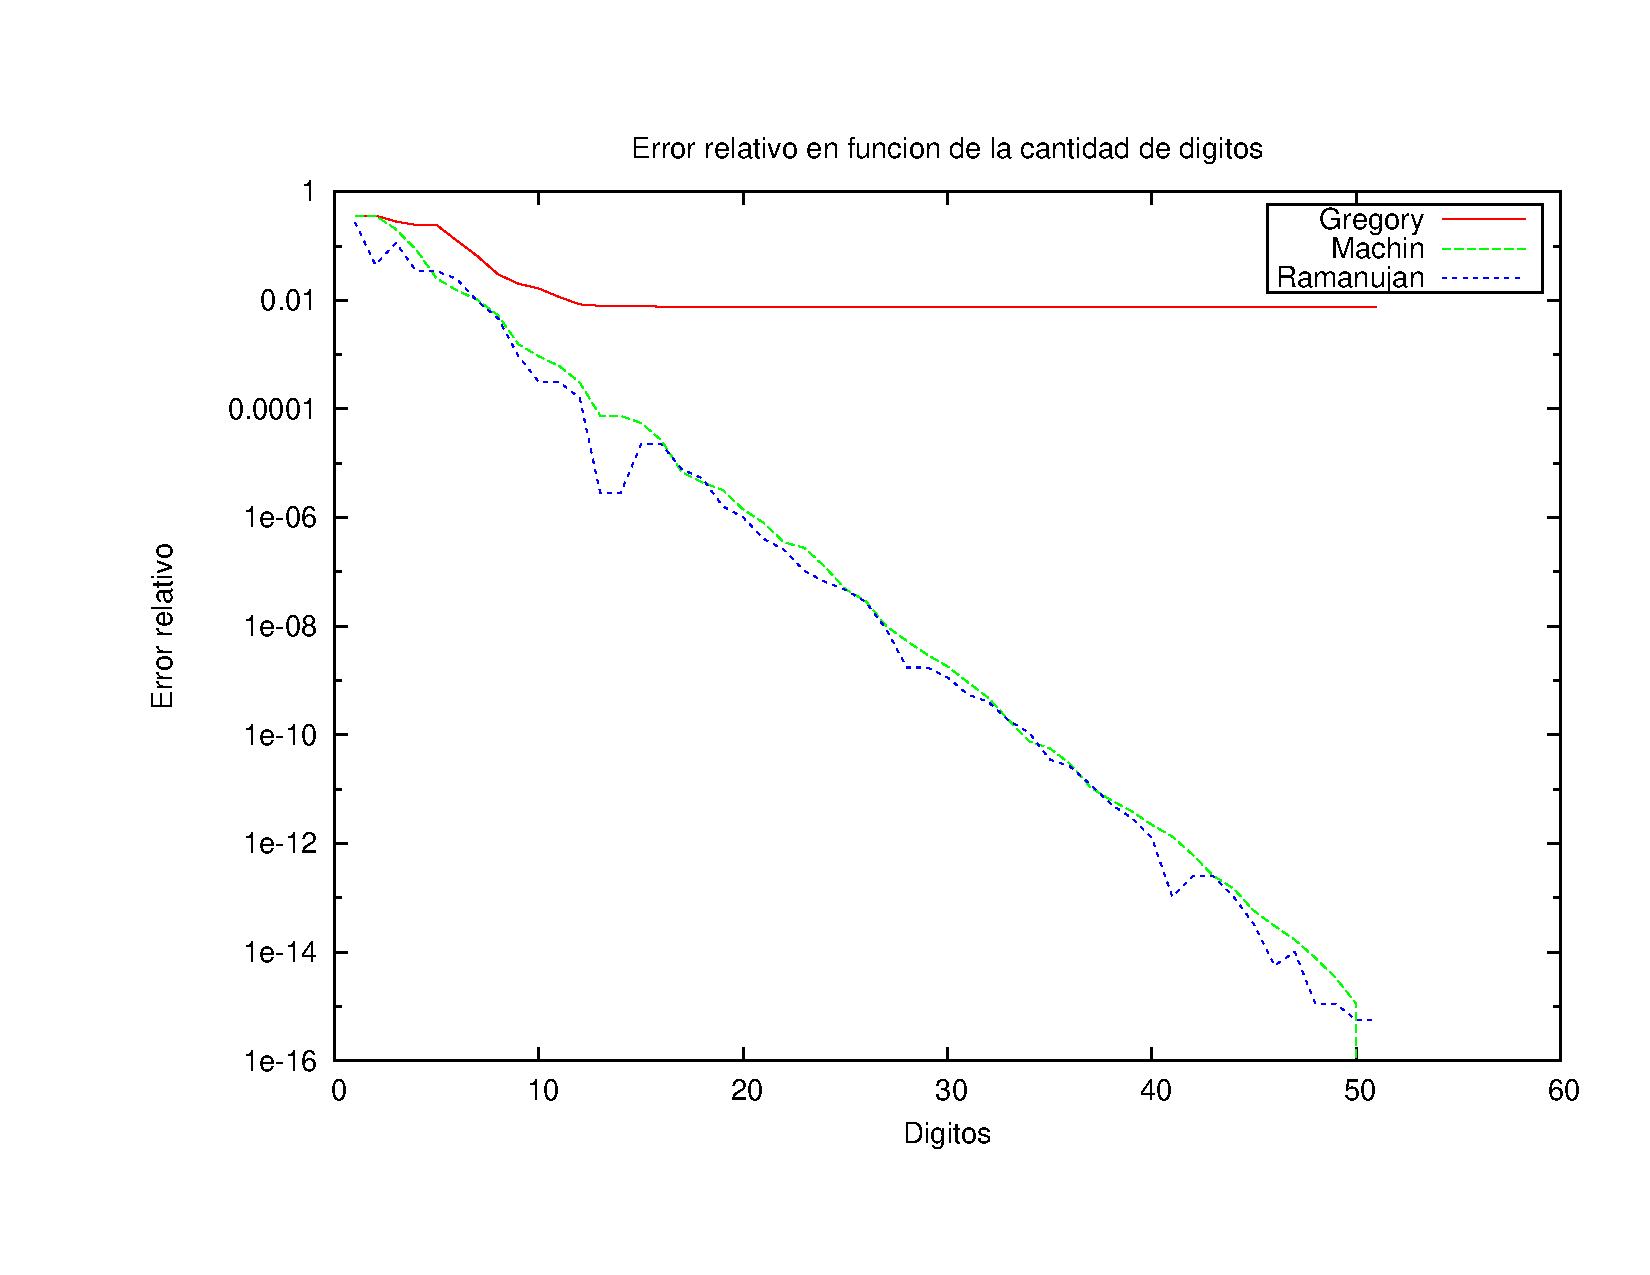
\includegraphics[width=14cm]{graficos/comparacion_42it_1a51p.pdf}
	  \caption{Comparación del error relativo de las tres series en el términos 42 variando de 1 y 51 la cantidad de bits en la mantisa.}
	  \label{fig:42it}
	\end{figure}
	
	\VSP
	
	La apreciación (lineal, exponencial, etc) de como decrecen los errores en función de la cantidad de dígitos es la misma que en función de la cantidad de iteraciones para $Gregory$ y $Machin$.
	
	$Ramanujan$ a diferencia de tener un 'error constante' alcanzado en pocas iteraciones como pasa en el gráfico anterior (51 digitos de presición), parece reducir de manera exponencial el error cometido conforme aumenta la presición utilizada.\\
	
	Observamos al igual que en el gráfico anterior que el error cometido por $Machin$ con 51 dígitos de presición no aparece graficado mientras que con el resto de las precisiones si. Concluimos a partir de esto, que a pesar que el error cometido por ambas series ($Machin$ y $Ramanujan$) es similar con 42 iteraciones, se necesita la máxima presicion brindada para que se haga totalmente despreciable la diferencia, si existe.\\

	Por otra parte, vemos que cuando la presición utilizada es baja (con la cantidad de iteraciones usada) las distintas series se comportan de manera similar. Realizamos otro gŕafico para ver que sucede con estas presiciones si la cantidad de terminos calculados es menor. Elegimos arbitrariamente correr las pruebas con 5 iteraciones.
	
	\begin{figure}[H]
	  \centering
		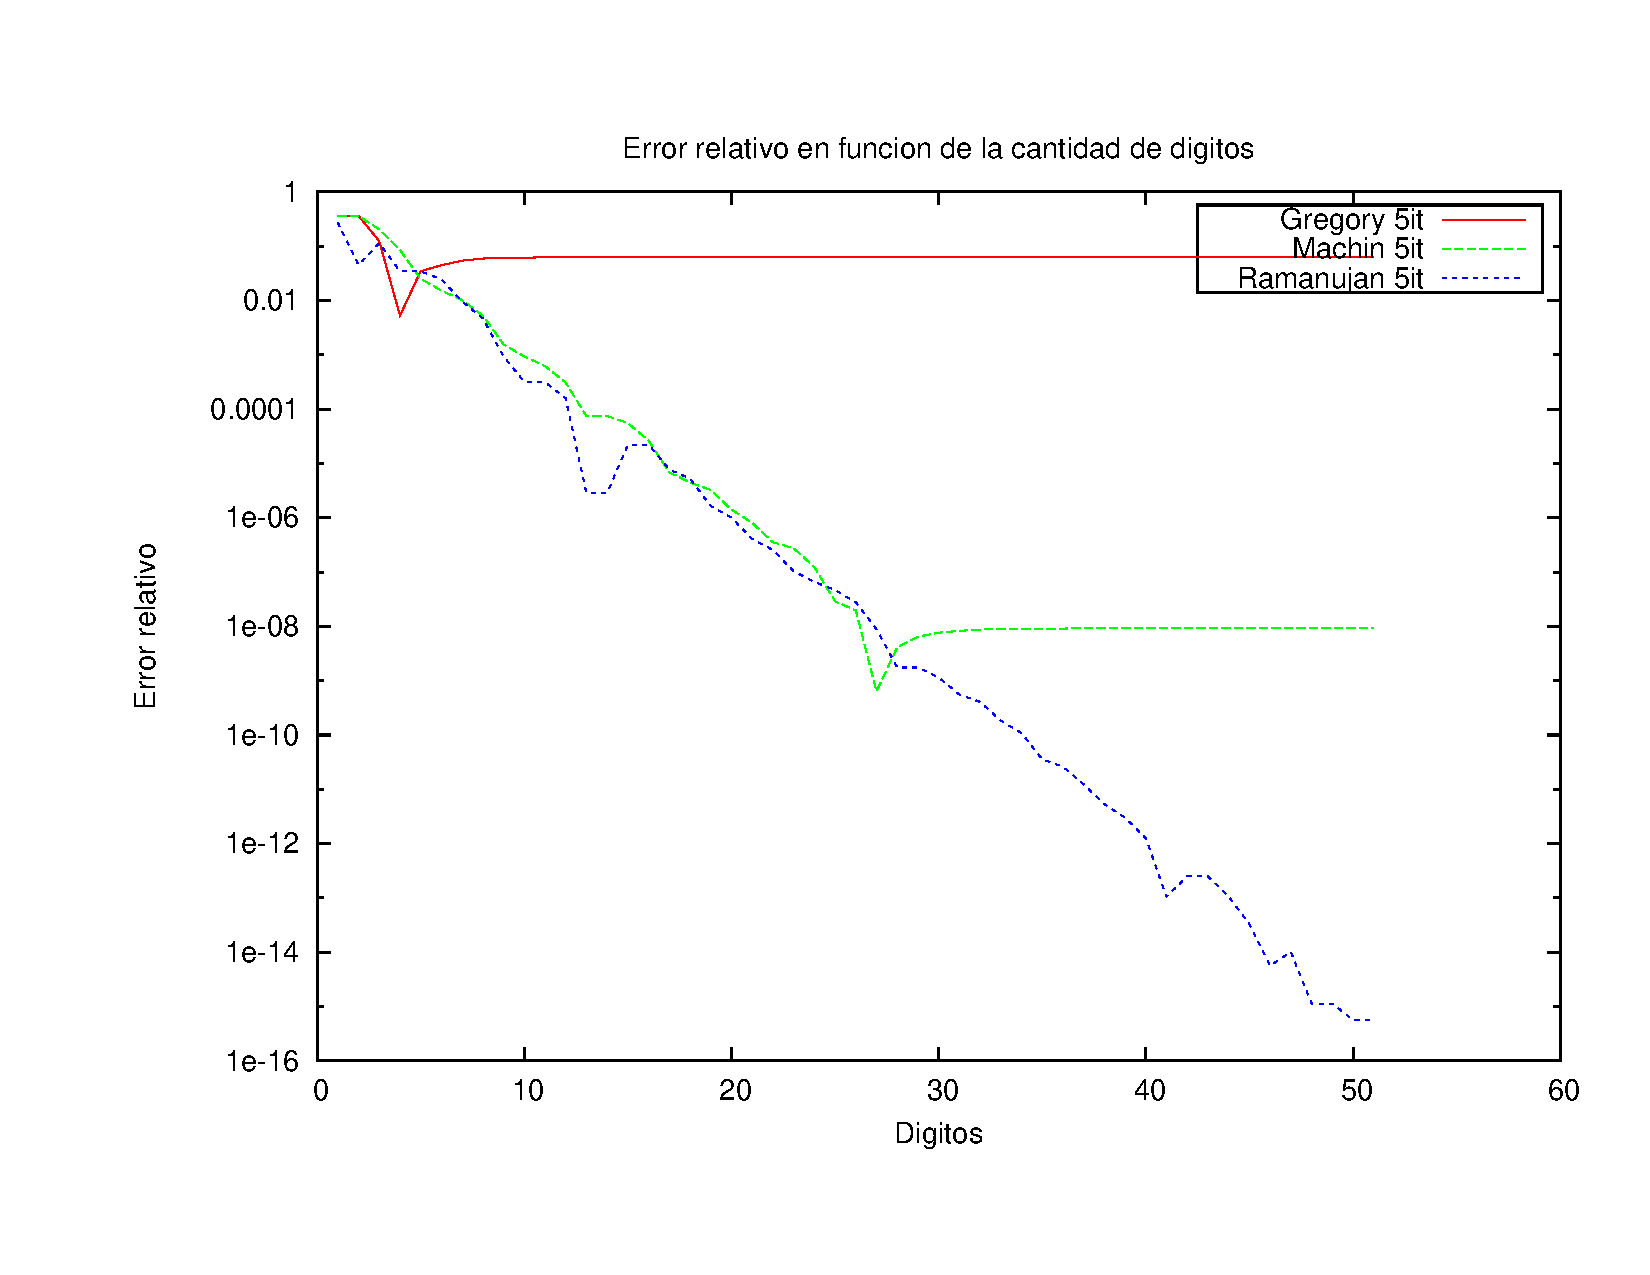
\includegraphics[width=14cm]{graficos/comparacion_5it_1a51p.pdf}
	  \caption{Comparación del error relativo de las tres series en el términos 5 variando de 1 y 51 la cantidad de bits en la mantisa.}
	  \label{fig:5it}
	\end{figure}
	
	\VSP
	
	Vemos que con poca presición los errores siguen siendo similares.
	
	Comparando este gráfico con el anterior podemos decir que la serie de $Gregory$ necesita de muchas iteraciones para poder alcanzar una 'buena' aproximación a $\pi$ ya que a pesar de ir aumentando la cantidad de dígitos utilizados la mejora en calidad de la aproximación empieza a ser despreciable cuando se alcanza una cantidad de dígitos.
	Como con menos iteraciones el error se 'estabiliza' (la diferencia en el error al aumentar los dígitos es despreciable) en una cantidad de dígitos menor, dicho error es mayor. Lo mismo ocurre con la fórmula de $Machin$ pero a mayor cantidad de dígitos. Creemos que esto ocurre porque como $Machin$ consigue mejores aproximaciones que $Gregory$ fijando una cantidad de iteraciones, cuando la presición es baja pierde mayor información al truncar lo que se ve reflejado en la diferencia de errores al aumentar dicha presición (necesita mas dígitos para estabilizarse).\\

	NOTA: No se utilizaron polinomios interpoladores para aproximar por la curva o recta que pase por todos los puntos correspondiente a una misma fuente de datos, estas conclusiones fueron sacadas utilizando experimentación empírica, suponiendo que el comportamiento cuando los valores del eje $x$ tienden a infinito se corresponden a los de los valores graficados.

\end{section}
